\section{Rails Web Servers} % (fold)
\label{tech:sec:rails_webservers}
In its simplest manner, a web server is a never ending \textit{loop} that accepts connections on listening \textit{socket} and handles them somehow. There are notorious differences on how this \textit{loop} is implemented, besides the classical architectural and philosophical differences behind each web server. These differ in handling multi processing, multi threading, asynchronous events, data copying, context switching, locking contention, memory management, blocking operations, HTTP parsing, the TCP stack implementation and many others.


\subsection{WEBrick}
This web server is Ruby's pioneer, created in 2000 by Masayoshi Takahashi and Yuuzou Gotou. WEBrick is a full-featured server that supports HTTP, HTTPS and listening concurrently to several ports, among other features. It is written in Ruby and has a very modular design, allowing developers to extend its functionalities by supporting external handlers~\cite{webrick_guide}.
WEBrick uses a single process but spawns a new thread for each incoming request. Since it is written in Ruby, its HTTP parser is known for its poor performance~\cite{ruby_webservers}. WEBrick's request handling is demonstrated on figure~\ref{fig:webrick_architecture}.
\begin{figure}[h]
  \centering
    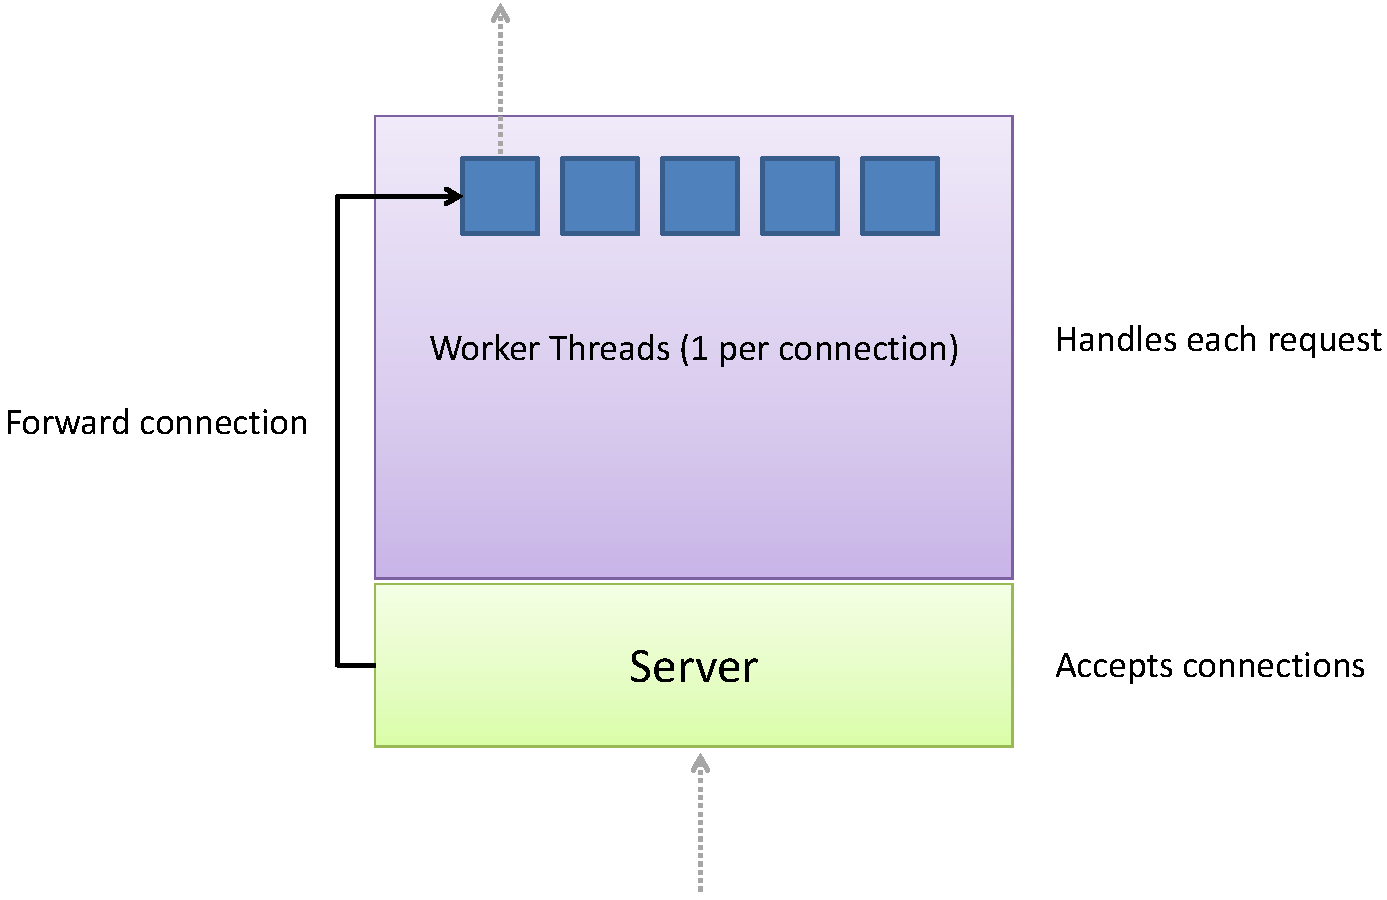
\includegraphics[width=0.75\textwidth]{webrick_architecture}
  \caption{WEBrick's request handling process}
  \label{fig:webrick_architecture}
\end{figure}
Due to its poor performance, users normally used alternate setups which were also known for their lacking stability~\cite{ruby_webservers}.


\subsection{Mongrel}
Mongrel was released by Zed A. Shaw in 2006 and soon became the most popular web server in Rails production environments. It offered much better performance when compared to WEBrick and it was reasonably suited for production environments. This was mainly due to its improved implementation of the HTTP parser, which was now written in C~\cite{mongrel_server_production}.

Similarly to WEBrick, Mongrel uses a single process. It has an acceptor thread which handles every incoming connection, launching new threads for each one of them. In production environments, Mongrel is commonly found in clustered configurations where several processes are launched and their usage is dictated by a proxy server~\cite{mongrel_faq}. Mongrel's request handling is demonstrated on figure~\ref{fig:mongrel_architecture}.
\begin{figure}[h]
  \centering
    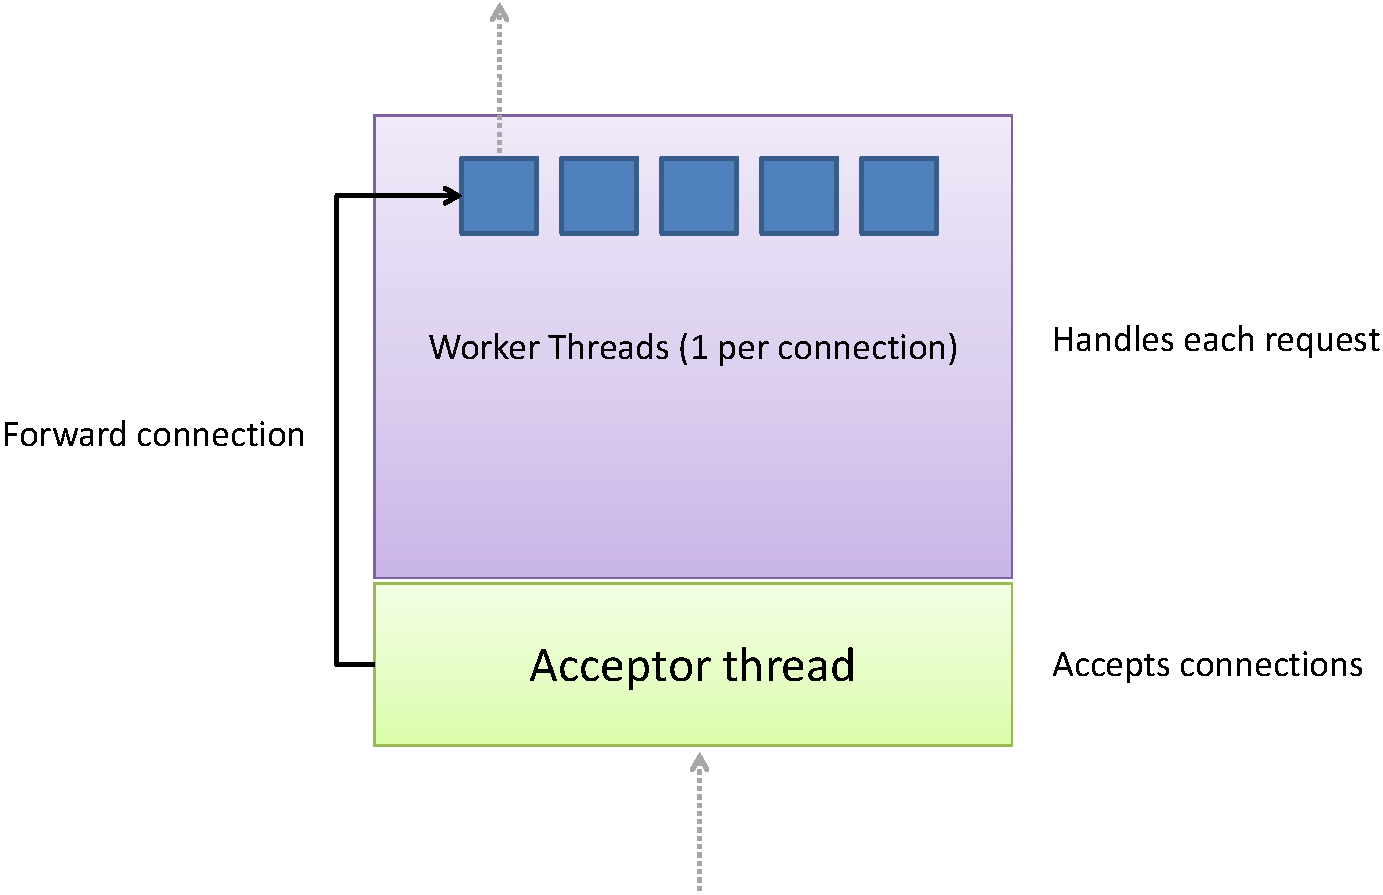
\includegraphics[width=0.75\textwidth]{mongrel_architecture}
  \caption{Mongrel's request handling process}
  \label{fig:mongrel_architecture}
\end{figure}
Mongrel also optimized the TCP stack by changing Ruby's default socket listening queue from 5 to 1024, besides using optimization flags on socket connections to improve bandwidth usage~\cite{mongrel_faq}.


\subsection{Thin}
Thin was released in 2008 and was the first Ruby web server which did not follow the \textit{one thread per request} convention. It uses Mongrel's HTTP parser and EventMachine as its I/O back-end, allowing it to use a fast asynchronous event loop in a single thread for all incoming requests~\cite{thin}. Thin recently became able to combine threading with its philosophy, by allowing the creation of a background pool of 20 threads~\cite{ruby_webservers}. Thin's request handling is demonstrated on figure~\ref{fig:thin_architecture}.
\begin{figure}[h]
  \centering
    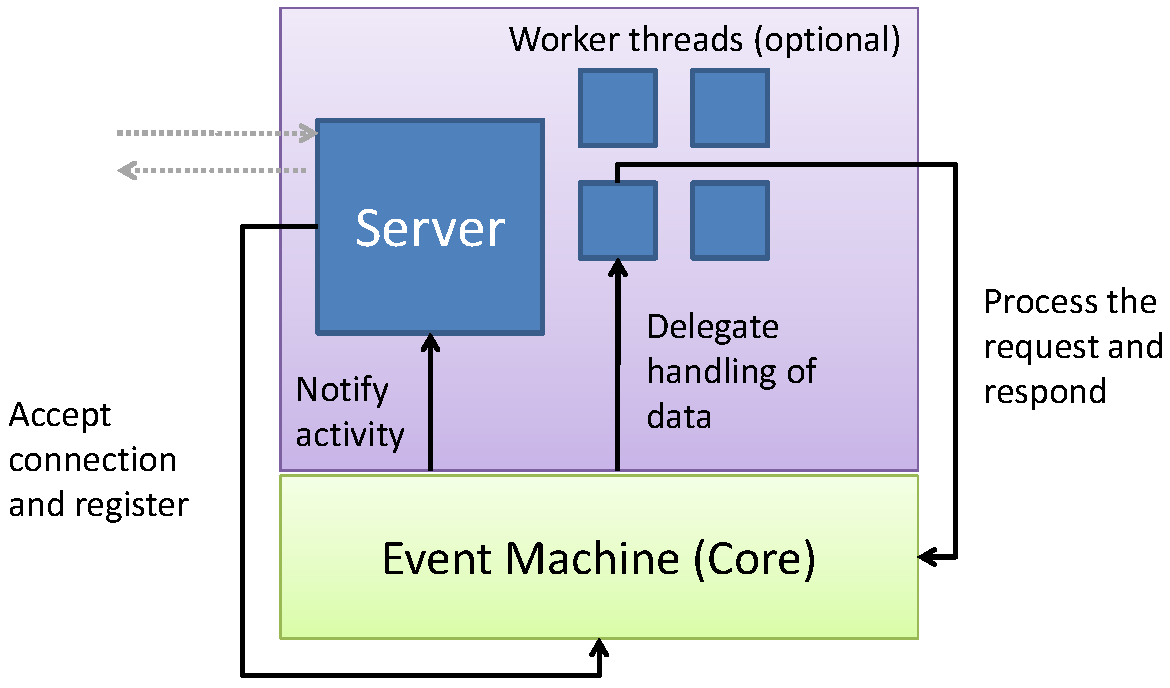
\includegraphics[width=0.75\textwidth]{thin_architecture}
  \caption{Thin's request handling process}
  \label{fig:thin_architecture}
\end{figure}
 This setup yields better performance and scalability than Mongrel, especially when serving small requests like, for example, API calls. This is mainly related to the fact that this web server does not launch a new thread for each request requiring less memory and no context switches~\cite{ruby_webservers}.


\subsection{Passenger}
Passenger was also released in 2008 but it had a big difference from the other options --- it was not a self-contained web server. Passenger relies on other web servers like Apache or Nginx by using their reliable web stack. It is used as a module or extension to these generic web servers, adding the needed functionality to support Ruby and handling certain types of requests~\cite{passenger_whatis}.

When the web server starts, having Passenger loaded as a module, it launches a Ruby process that will be responsible for all the other processes handling the Ruby application, called the \textit{worker processes}. Each request is delivered to the firstly created Ruby processes, which forwards it to one of its worker threads. These worker processes are single threaded and handle one request at a time~\cite{ruby_webservers}. Passenger's request handling is demonstrated on figure~\ref{fig:passenger_architecture}.
\begin{figure}[h]
  \centering
    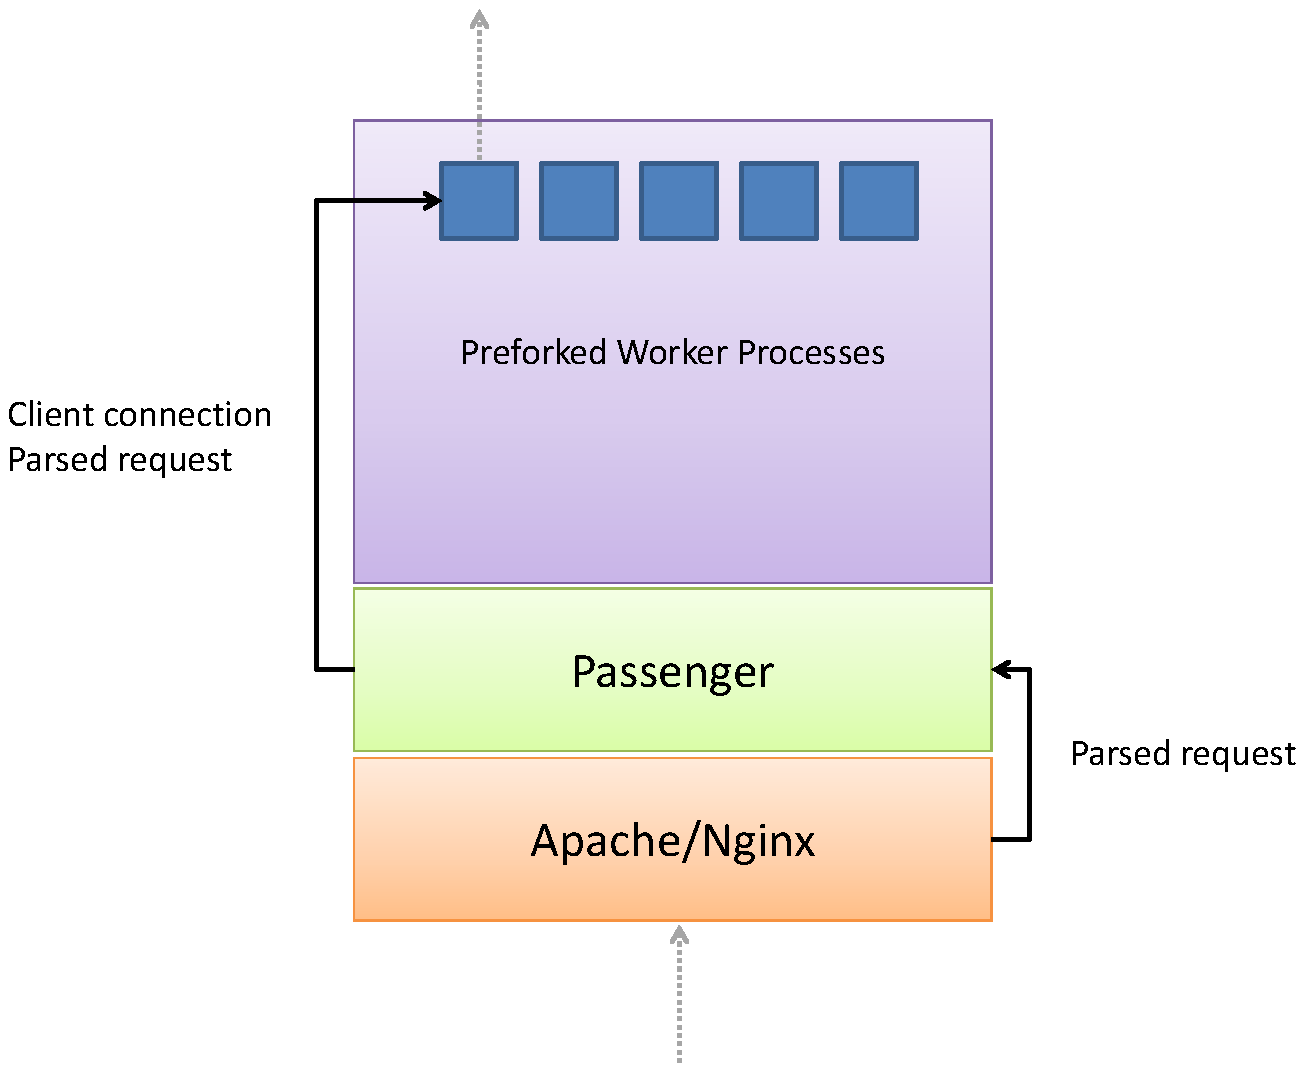
\includegraphics[width=0.75\textwidth]{passenger_architecture}
  \caption{Passenger's request handling process}
  \label{fig:passenger_architecture}
\end{figure}
Passenger is the first real multi-process server for Ruby, although setups with multiple Mongrel or Thin servers were already being used~\cite{passenger_whatis}. Passenger is free but Phusion also provides commercial support.


\subsubsection{Apache}
The Apache HTTP Server is a full-featured and open source web server created by the Apache Software Foundation. It consists on a general purpose web server and provides many useful features such as HTTPS, IPV6 and authentication. Apache natively handles many web development languages such as PHP and Perl~\cite{apache_features}. It can be extended with modules and this is where Passenger comes in --- it will act as \textit{mod\_rails} and extend Apache's functionality to be able to handle Ruby on Rails' applications~\cite{passenger_whatis}.


\subsubsection{Nginx}
Nginx is a lightweight open source web server with a strong focus on performance created by Igor Sysoev~\cite{nginx_features}. Passenger can extend Nginx's functionality by being installed as its module, similarly to the Apache's procedure~\cite{passenger_whatis}.
